%%%%%%%%%%%%%%%%%%%%%%%%%%%%%%%%%%%%%%%%%%%%%%%%%%%%%%%%%%%
% Szablon ksi��ki
% Autor: Tomasz Kubik
% udost�pniany na prawach CreativeCommons: SA-BY-NC
%
%
%%%%%%%%%%%%%%%%%%%%%%%%%%%%%%%%%%%%%%%%%%%%%%%%%%%%%%%%%%%
\documentclass[a4paper,11pt,polish]{memoir}
% acelnosxz
% ����󶼿
% ��ʣ�Ӧ��
%%%%%%%%%%%%%%%%%%%%%%%%%%%%%%%%%%%%%%%%%%%%%%%%%%%%%%%%%%%%
%%    Pakiety podstawowe                                  %%
%%%%%%%%%%%%%%%%%%%%%%%%%%%%%%%%%%%%%%%%%%%%%%%%%%%%%%%%%%%%
\usepackage[cp1250]{inputenc} %ustawienie kodowania znak�w
\usepackage[T1]{fontenc}
\usepackage{pslatex}
\usepackage[polish]{babel}
\usepackage{tabularx}
\usepackage{multicol}
\usepackage{color,colortbl}
\usepackage{calc,soul,fourier}
\usepackage{setspace}
\usepackage{indentfirst}
\usepackage{type1cm,eso-pic}
\usepackage{ifpdf}
\usepackage{amsmath}  
\usepackage{listings}
\usepackage{longtable}
\usepackage{url}

%%%%%%%%%%%%%%%%%%%%%%%%%%%%%%%%%%%%%%%%%%%%%%%%%%%%%%%%%%%%
%%    Pakiety dodatkowe                                   %%
%%%%%%%%%%%%%%%%%%%%%%%%%%%%%%%%%%%%%%%%%%%%%%%%%%%%%%%%%%%%
%\RequirePackage[caption=false,position=bottom]{subfig} 
%\let\subbottom\subfloat
%\usepackage[version=3]{mhchem}

%%%%%%%%%%%%%%%%%%%%%%%%%%%%%%%%%%%%%%%%%%%%%%%%%%%%%%%%%%%%
%%    Pakiety do bibliografii i importu grafiki           %%
%%%%%%%%%%%%%%%%%%%%%%%%%%%%%%%%%%%%%%%%%%%%%%%%%%%%%%%%%%%%
\usepackage[sectionbib]{chapterbib}
\makeatletter
\renewcommand{\@memb@bsec}{\section*{\bibname}\prebibhook}
\makeatother

\usepackage{makeidx} \makeindex 
\ifpdf
 \usepackage[pdftex,bookmarks,breaklinks,unicode]{hyperref}
 \usepackage[pdftex]{graphicx}
 \DeclareGraphicsExtensions{.pdf,.jpg,.mps,.png}
 \pdfcompresslevel=9
\else
 \usepackage{graphicx}
 \DeclareGraphicsExtensions{.eps,.ps,.jpg,.mps,.png}
\fi

%%%%%%%%%%%%%%%%%%%%%%%%%%%%%%%%%%%%%%%%%%%%%%%%%%%%%%%%%%%%
%%    Znaczniki ci�cia                                    %%
%%%%%%%%%%%%%%%%%%%%%%%%%%%%%%%%%%%%%%%%%%%%%%%%%%%%%%%%%%%%
\makeatletter
\AddToShipoutPicture{%
  \setlength{\unitlength}{1mm}
%% 162 x 234
  \put(18,31.5){\line(-1,0){10}}%29.5
  \put(24,26.5){\line(0,-1){10}}%21
  \put(192,31.5){\line(1,0){10}}%29.5
  \put(186,26.5){\line(0,-1){10}}%189
  \put(18,265.5){\line(-1,0){10}}%267.5
  \put(24,270.5){\line(0,1){10}}%21
  \put(192,265.5){\line(1,0){10}}%267.5
  \put(186,270.5){\line(0,1){10}}%189
%% 168 x 238
 \put(18,29.5){\line(-1,0){10}}%
  \put(21,26.5){\line(0,-1){10}}%
  \put(192,29.5){\line(1,0){10}}%
  \put(189,26.5){\line(0,-1){10}}%
  \put(18,267.5){\line(-1,0){10}}%
  \put(21,270.5){\line(0,1){10}}%
  \put(192,267.5){\line(1,0){10}}%
  \put(189,270.5){\line(0,1){10}}%
}
\makeatother

%%%%%%%%%%%%%%%%%%%%%%%%%%%%%%%%%%%%%%%%%%%%%%%%%%%%%%%%%%%%
%%    Ustawienia strony + definicje pomocnicze            %%
%%%%%%%%%%%%%%%%%%%%%%%%%%%%%%%%%%%%%%%%%%%%%%%%%%%%%%%%%%%%
\setlength{\headsep}{9pt} 
%\setlength{\headheight}{0pt}
\setlength{\hoffset}{0mm} %%a4
\setlength{\voffset}{0mm} %-14mm %%a4
\setlength{\footskip}{23pt} % 23pt ~= 8mm
\setlength{\topmargin}{13mm}%{7.65mm} %28pt -2.5mm
%\setlength{\oddsidemargin}{11.85mm}
%\setlength{\evensidemargin}{11.85mm}
%\setlength{\textwidth}{135.5mm}
%\setlength{\textheight}{203.6mm}

\setlength{\parindent}{15pt}
\setlength{\parskip}{0pt} %{1ex plus 0.5ex minus 0.2ex}
\newlength\mytemplengtha

\setlength{\extrarowheight}{2pt}
%\setlength{\topmargin}{8mm}%{7.65mm} %28pt -2.5mm
\setlength{\oddsidemargin}{15mm}
\setlength{\evensidemargin}{15mm}
\setlength{\textwidth}{129mm}%135.5
\setlength{\textheight}{201mm}%203.6
%\setlength{\parindent}{16pt}%18


\sloppy  % wyr�wnanie z dw�ch stron
\renewcommand{\topfraction}{1.0}
\renewcommand{\bottomfraction}{1.0}
\renewcommand{\textfraction}{0.0}

\widowpenalty=10000 % ostatni wiersz akapitu nie zostanie przeniesiony na nast?pn? stron? 
\clubpenalty=10000 % pierwszy wiersz akapitu nie b?dzie ko?czy? strony (nie u?ywam tego ustawienia)
%\tolerance = 500 \pretolerance = 900 %% sk?ad z wi?ksz? `tolerancj?' (mo?na te warto?ci zwi?kszy? bardziej)
%\hbadness= 1450 %% zmniejsza licz? wy?wietlanych ostrze?e? (mo?na zwi?kszy?, ale bez przesady)
%\hfuzz = 1.5pt %% tekst mo?e stercze? ma marginesie na 1,5pt (ok. 0,5mm)

\setlength\floatsep{6pt plus 2pt minus 2pt} 
\setlength\intextsep{12pt plus 2pt minus 2pt} 
\setlength\textfloatsep{12pt plus 2pt minus 2pt} 
%\captionnamefont{\small\bfseries}
%\captiontitlefont{\small}
\setbeforesecskip{10pt plus 0.5ex}%{-3.5ex \@plus -1ex \@minus -.2ex}
\setaftersecskip{10pt plus 0.5ex}%\onelineskip}
\setbeforesubsecskip{8pt plus 0.5ex}%{-3.5ex \@plus -1ex \@minus -.2ex}
\setaftersubsecskip{8pt plus 0.5ex}%\onelineskip}

%\setlength{\floatsep}{12pt}
%\setlength{\textfloatsep}{12pt}
%\setlength{\intextsep}{12pt}
%\setlength{\arrayrulewidth}{0.5pt}
\usepackage{color}
\definecolor{lightgray}{rgb}{.9,.9,.9}
\definecolor{darkgray}{rgb}{.4,.4,.4}
\definecolor{purple}{rgb}{0.65, 0.12, 0.82}
%\definecolor{nicered}{rgb}{.647,.129,.149}
\definecolor{nicered}{rgb}{.0,.0,.0}

%%%%%%%%%%%%%%%%%%%%%%%%%%%%%%%%%%%%%%%%%%%%%%%%%%%%%%%%%%%%
%%    Zmienione otoczenia                                 %%
%%%%%%%%%%%%%%%%%%%%%%%%%%%%%%%%%%%%%%%%%%%%%%%%%%%%%%%%%%%%
\makeatletter
\renewenvironment{itemize}{
  \begin{list}{  
  \csname labelitem\romannumeral\the\@listdepth\endcsname}{
  \setlength{\leftmargin}{1em}
	\setlength{\topsep}{6pt}%
	\setlength{\partopsep}{0pt}%
	\setlength{\parskip}{0pt}%
	\setlength{\parsep}{0pt}%
	\setlength{\itemsep}{0pt}}
}{
  \end{list}
}
\renewenvironment{quote}{
  \begin{list}{}{}
	 \item[]}
	 {\unskip\end{list}}
\makeatother

\setlength{\leftmargini}{1.5em}
\usepackage{bibspacing}
\setlength{\bibspacing}{\baselineskip}

\makeatletter
\newskip\@hlskip
%\@hlskip=.5\baselineskip \@plus 1mm \@minus .5mm
\@hlskip=6pt

\newdimen\verbatimleftmargin
  \verbatimleftmargin\z@
\newdimen\verbatimbaselineskip
  \verbatimbaselineskip\baselineskip
\def\verbatimsize{\normalsize}

\def\@verbatim{%
 \topsep\@hlskip
 \partopsep\z@\parsep\z@\itemsep\z@
 \trivlist \item\relax
  \if@minipage\else
   \vskip\baselineskip
   \vskip-\verbatimbaselineskip
%  \vskip\parskip
  \fi
  \leftskip\@totalleftmargin
  \if@minipage\else
   \advance \leftskip by \verbatimleftmargin
  \fi
  \rightskip\z@skip
  \parindent\z@\parfillskip\@flushglue\parskip\z@skip
  \@@par
  \@tempswafalse
  \def\par{%
    \if@tempswa
      \leavevmode \null \@@par\penalty\interlinepenalty
    \else
      \@tempswatrue
      \ifhmode\@@par\penalty\interlinepenalty\fi
    \fi}%
  \let\do\@makeother \dospecials
  \obeylines 
   \verbatimsize \baselineskip\verbatimbaselineskip
   \verbatim@font \@noligs
  \everypar \expandafter{\the\everypar \unpenalty}%
}
\makeatother


\newcommand{\autorzy}{}

\makeatletter
\newlength\dlf@normtxtw
\setlength\dlf@normtxtw{\textwidth}
\def\myhelvetfont{\def\sfdefault{mdput}}
\newsavebox{\feline@chapter}
\newcommand\feline@chapter@marker[1][4cm]{%
\sbox\feline@chapter{%
\resizebox{!}{#1}{\fboxsep=1pt%
\colorbox{nicered}{\color{white}\bfseries\sffamily\thechapter}%
}}%
\rotatebox{90}{%
\resizebox{%
\heightof{\usebox{\feline@chapter}}+\depthof{\usebox{\feline@chapter}}}%
{!}{\scshape\so\@chapapp}}\quad%
\raisebox{\depthof{\usebox{\feline@chapter}}}{\usebox{\feline@chapter}}%
}
\newcommand\feline@chm[1][4cm]{%
\sbox\feline@chapter{\feline@chapter@marker[#1]}%
\makebox[0pt][l]{% aka \rlap
\makebox[1cm][r]{\usebox\feline@chapter}%
}}
\makechapterstyle{daleif1}{
\renewcommand\chapnamefont{\normalfont\Large\scshape\raggedleft\so}
\renewcommand\chaptitlefont{\normalfont\huge\bfseries\scshape\color{nicered}}
\renewcommand\chapternamenum{}
\renewcommand\printchaptername{}
\renewcommand\printchapternum{\vspace{-3cm}\null\hfill\feline@chm[2.5cm]\par}
\renewcommand\afterchapternum{\par\vskip\midchapskip}
\renewcommand\printchaptertitle[1]{\chaptitlefont\raggedleft ##1\\  \makebox[\textwidth - (1cm + \widthof{\Huge \thechapter.})][r]{\Large \itshape \autorzy}\par}
}

\addtopsmarks{headings}{%
\nouppercaseheads % added at the beginning
}{%
\createmark{chapter} {left}{shownumber}{}{. \space}
\createmark{section}{right}{shownumber}{}{. \space}
}%use the new settings
\pagestyle{headings}

\setcounter{secnumdepth}{2}
\setcounter{tocdepth}{2}
\setsecnumdepth{subsection} % activating subsubsec numbering in doc


%definicja nag��wk�w
\copypagestyle{outer}{headings}
\makeoddhead{outer}{}{}{\small\color{nicered}\slshape\rightmark}
\makeevenhead{outer}{\small\color{nicered}\slshape\leftmark}{}{}
\makeoddfoot{outer}{}{}{\thepage}
\makeevenfoot{outer}{\thepage}{}{}
% fix plain
%\copypagestyle{plain}{outer} % overwrite plain with outer
\makeoddhead{plain}{}{}{} % remove right header
\makeevenhead{plain}{}{}{} % remove left header
\makeevenfoot{plain}{}{}{}
\makeoddfoot{plain}{}{}{}

\makepagestyle{intro}
\makeoddhead{intro}{}{}{\small\color{nicered}\slshape S�owo wst�pne}
\makeevenhead{intro}{\small\color{nicered}\slshape S�owo wst�pne}{}{}
\makeoddfoot{intro}{}{}{\thepage}
\makeevenfoot{intro}{\thepage}{}{}

%\renewcommand{\chaptermark}[1]{\markboth{\ifnum \c@secnumdepth >\z@ \thechapter \ \fi #1}{}} 
%\renewcommand{\chaptermark}[1]{\markboth{\thechapter \ #1}{\thesection \ #1}} 
%\renewcommand{\sectionmark}[1]{\markright{\thesection \ #1}{}} 
%\renewcommand{\chaptermark}[1]{\markboth{\thechapter \MakeUppercase{#1}}{}}

%kropki po numerach sekcji
\makeatletter
\def\@seccntformat#1{\csname the#1\endcsname.\quad}
\def\numberline#1{\hb@xt@\@tempdima{#1\if&#1&\else.\fi\hfil}}
\makeatother

% z jakiego? powodu czcionki s? mniejsze o jeden punkt ni? wynika?oby to z poni?szych ustawie?
\renewcommand{\bfdefault}{b}
\renewcommand{\normalsize}{\fontsize{11pt}{12.5pt}\selectfont}
\newcommand{\smallp}{\fontsize{9.5pt}{11.5pt}\selectfont}
\makeatother

%Podpisy pod rysunkami i tabelami
%\AtBeginDocument{% 
        \addto\captionspolish{% 
        \renewcommand{\tablename}{Tab.}% 
}%} 
%\AtBeginDocument{% 
%        \addto\captionspolish{% 
%        \renewcommand{\chaptername}{Rozdzia�}% 
%}} 

%\AtBeginDocument{% 
        \addto\captionspolish{% 
        \renewcommand{\figurename}{Rys.}% 
}%}

%%% Strona tytu?owa
%%% Strona tytu�owa
\newcommand*{\titleTH}{\begingroup% T&H Typography
\raggedleft
\vspace*{5cm}
{\textcolor{nicered}{\fontsize{28}{28}\fontfamily{put}\bfseries\selectfont 	KOMPUTEROWE}}\\[\baselineskip]
{\textcolor{nicered}{\fontsize{28}{28}\fontfamily{put}\bfseries\selectfont 	PRZETWARZANIE}}\\[\baselineskip]
{\textcolor{nicered}{\fontsize{28}{28}\fontfamily{put}\bfseries\selectfont 	WIEDZY}}\\[2cm]
{\fontsize{18}{18}\fontfamily{put}\bfseries\selectfont Kolekcja prac 2012/2013}\\[0.5\baselineskip]
{\fontsize{18}{18}\fontfamily{put}\bfseries\selectfont pod redakcj� Tomasza Kubika}\\
\vfill
%{\Large Politechnika Wroc�awska, 2011}\par
\vspace*{3\baselineskip}
\endgroup}


%\counterwithout{figure}{chapter}
%\counterwithout{table}{chapter}


\begin{document}
\pagestyle{outer}
\openany
\chapterstyle{daleif1}
\thispagestyle{empty} \pdfbookmark[0]{Tytu�}{Tytul.1}\titleTH \clearpage

\mbox{}\pdfbookmark[0]{Spis tre�ci}{spisTresci.1}
\tableofcontents*
%\thispagestyle{empty} 
\cleardoublepage

\pagestyle{outer}
\bibliographystyle{plunsrt}
\renewcommand{\autorzy}{M.~Nowak, G.~Maj}
\chapter[Audyt w systemach informatycznych][Audyt w systemach informatycznych]{Audyt w systemach informatycznych}

  Jednym z podstawowych problem�w profesjonalnego zarz�dzania firm� w~bran�y informatycznej jest zarz�dzanie jako�ci�. Jako�� mo�na definiowa� i mierzy� na wielu poziomach. Bardzo du�o uwagi po�wi�cane jest jako�ci produkt�w, cho� r�wnie wa�nym elementem jest ocena jako�ci pracy pracownik�w oraz ich efektywno�ci. Audyt w systemach informatycznych powinien zawiera� tak�e elementy oceny jako�ci pracy i s�u�y� usprawnieniu dzia�ania organizacji.

W rozwa�aniach na temat oceny jako�ci pracy i wydajno�ci pracownik�w skupiono si� na firmach informatycznych, kt�rych przedmiotem dzia�alno�ci jest wytwarzanie oprogramowania. Kluczowym pracownikiem bior�cym udzia� w tworzeniu ko�cowego produktu, czyli programu jest programista. Ocena pracy programisty jest zadaniem z�o�onym i wymaga znajomo�ci wielu aspekt�w procesu wytwarzania oprogramowania. W dzisiejszych czasach zarz�dzanie jako�ci� oprogramowania jest prawdziwym wyzwaniem dla du�ych firm o zasi�gu globalnym zatrudniaj�cych tysi�ce programist�w z ca�ego �wiata.

Podstawowym pytaniem, kt�re postawiono w tym rozdziale jest: jak efektywnie mierzy� jako�� i efektywno�� pracy programisty? W niniejszym artykule autorzy postaraj� si� przybli�y� problem, przedstawi� dost�pne na rynku rozwi�zania oraz opisa� prosty system kontroli efektywno�ci pracy.


\section{Dost�pne systemy pomiaru pracy}
\label{sec:dostepneSystemy}

Na rynku istniej� r�ne systemy s�u��ce do pomiaru i wspomagania pracy programisty. Skupiaj� si� one
g��wnie na ��czeniu kodu i kontroli pracy wielu programist�w, pracuj�cych nad jednym projektem. Poni�ej przedstawione zosta�y najpopularniejsze systemy, w tym rozbudowane i szeroko wykorzystywane systemy otwarto�r�d�owe.

\subsection{Systemy kontroli wersji}
Przyk�adami system�w kontroli wersji s� najbardziej popularne darmowe systemy takie jak:
\begin{itemize}
	\item Git,
	\item Svn,
	\item Mercurial.
\end{itemize}

Systemy kontroli wersji stworzone s� do pomocy przy rozwoju oprogramowania, ich g��wnym zadaniem jest ��czenie pracy wielu pracownik�w jednego projektu, jednak poprzez tworzenie historii zmian w projekcie daje mo�liwo�� kontroli i oceny pracy pracownik�w.
Daj� one mo�liwo�� �ledzenia post�pu prac poczynionych przez poszczeg�lnych pracownik�w. Podstawowe informacje, kt�re mo�na uzyska� to:
\begin{itemize}
	\item jaki u�ytkownik i kiedy wprowadza� zmiany,
	\item mo�liwo�� sprawdzenia jakie zmiany zosta�y wprowadzone w danym commicie:
	\begin{itemize}
		\item dok�adne r�nice mi�dzy zmienionymi plikami,
		\item skr�cone statystyki(ilo�� zmian bez poszczeg�lnych r�nic),
		\item sumy kontrolne poszczeg�lnych zmian,
		\item wy�wietlanie tylko informacji przez nas okre�lonych,
	\end{itemize}
	
	\item mo�liwo�� dostosowania informacji przez nas �ledzonej: 
	\begin{itemize}
		\item kontrola jednego pracownika,
		\item kontrola danego okresu zmian,
		\item kontrola historii tworzenia i ��czenia ga��zi.
	\end{itemize}

\end{itemize}


	\subsubsection{Git}
	Git jest rozproszonym systemem kontroli wersji. Jest to wolne oprogramowanie udost�pnione na licencji GNU GPL2. Git powsta� jako alternatywa dla zamkni�tego systemu BitKeeper w kwietniu 2005 roku do rowijania projektu Linux.
	
	\subsubsection{Svn}
	Subversion jest wolnym syetmem kontroli wersji udost�pnionym na licencji Apache. Zosta� stworzony do zast�pienia systemu CVS.
	
	\subsubsection{Mercurial}
	Marcurial podobnie jak Git jest rozproszonym systemem kontroli wersji. Zosta� napisany w tym samym czasie jak Git, te� w celu pomocy do rozwijania projektu Linux. Jest wykorzystywany w wielu projektach otwarto�r�d�owych.

\subsection{Systemy zarz�dzania projektem}

\begin{itemize}
	\item Redmine
	
	Redmine je� wolnym, otwarto�r�d�owym internetowym narz�dziem do zarz�dzania projektem i szukania
	b��d�w. Udost�pnia kalendarz i wykres Ganta wraz ze wsparciem wizualnym by �atwiej kontrolowa�
	ko�cz�ce si� etapy projektu. Wspiera r�ne systemy kontroli wersji i umo�liwia kontrole nad podzia�em
	zada� w grupie. Narz�dzie Redmine jest oparte o framework Ruby on Rails, co zapewnia mu przeno�no��.

	
	\item Jira
	
	JIRA jest zamkni�tym oprogramowaniem stworzonym przez firm� Atlassian, kt�re ma na celu wspomaganie w
	zarz�dzaniu projektem i �ledzeniu b��d�w. Jest wykorzystywana w wielu projektach m.in. Fedora
	Commons, Skype czy JBoss. Jest narz�dziem wieloplatformowym dzi�ki oparciu go o j�zyk Java. Firma
	Atlassian  udost�pnia program JIRA nieodp�atnie do u�ytku non-profit.


	\item GitHub.
	
	GitHub jest serwisem hostingowym dla projekt�w wykorzystuj�cych system kontroli wersji Git. Udost�pnia
	darmowe otwarte repozytoria a tak�e p�atne repozytoria zamkni�te. Opr�cz podstawowego zadania jakim
	jest przechowywanie plik�w projektu wspomaga kontrol� nad tworzeniem oprogramowania poprzez dodatkowe
	narz�dzie nieobecne w systemie Git np. bugtracker, forki repozytori�w, graficzne statystyki czy wiki z
	dokumentacj�. Umo�liwia ��czenie programist�w w organizacje i przydzielanie mo�liwo�ci rozwijania 
	oprogramowania dla konkretnych u�ytkownik�w.

\end{itemize}

\subsection{Systemy do statycznej analizy kodu}

\begin{itemize}
	\item Klocwork,
	
	Klockwork jest zamkni�tym programem przeznaczonym do statycznej ana lizy kodu pozwalaj�cym na detekcj�
	b��d�w strukturalnych kodu i b��d�w przebiegu programu. Umo�liwia prac� z najpopularniejszymi j�zykami
	C, C++, Java czy C#.
		 
	\item Pylint,
	
	Pylint jest otwrto�r�d�owym oprogramowaniem do znajdywania b��d�w w kodzie i sprawdzania jego jako�ci.
	Pylint jest podobny do innego oprogramowania Pychecker ale jest bardziej rozbudowany. Wspiera mi�dzy
	innymi sprawdzanie d�ugo�ci linii, sprawdzanie zgodno�ci nazw zmiennych ze standardem kodowania czy 
	tworzenie diagram�w UML ze stworzonego kodu.
	
	\item CodeSonar,
	
	CodeSonar jest zamkni�tym oprogramowaniem analizuj�cym kod poz wzgl�dem bezpiecze�stwa i poprawno�ci.
	Wspiera oprogramowanie napisane w C, C++ i Java. Jest wykorzystywany w wielu ga��ziach gospodarki
	m.in. w NASA czy w firmie Toyota. Opr�cz analizy kody umo�liwia wizualizacj� architektury programu i
	zbiera dane do metryk oceny jako�ci kodu.
	
\end{itemize}


\section[Sposoby pomiaru jako�ci pracy programisty][Sposoby pomiaru jako�ci pracy programisty]
{Sposoby pomiaru jako�ci pracy programisty}
\label{sec:sposobyPomiaruJakosci}
Na ocen� pracownika programisty mo�na patrze� z r�nych perspektyw. Z jednej strony, efektem jego
pracy jest kod �r�d�owy, wi�c podstawowym sk�adnikiem oceny powinna by� jego jako��. Z drugiej
strony jednak, w ka�dym projekcie obecne s� pewne ograniczenia czasowe, wi�c szybko�� pracy
pracownika jest r�wnie� wa�nym aspektem oceny. W og�lno�ci mo�na powiedzie�, �e jako�� pracy
programisty mo�na sprowadzi� do dw�ch sk�adnik�w:
\begin{itemize}
	\item oceny jako�ci kodu,
	\item oceny organizacji pracy.
\end{itemize}

Normy dotycz�ce zarz�dzania jako�ci� (np. ISO 9000:2008, ISO 15504-4:2005) definiuj� tzw. kluczowe 
wska�niki efektywno�ci (ang. KPI - key performance indicator). Wa�n� cech� tych wska�nik�w jest
to, �e opisuj� one mierzalne procesy w postaci liczbowej. Daje to mened�erowi obiektywny obraz
efektywno�ci danego procesu w przedsi�biorstwie i pozwala na cykliczn� kontrol� jako�ci. Poni�ej
przedstawiono kilka przyk�adowych wska�nik�w, kt�re spe�niaj� warunek mierzalno�ci, wi�c kwalifikuj�
si� do grupy KPI. 

\subsection[Ocena jako�ci wygenerowanego kodu][Ocena jako�ci wygenerowanego kodu]{Ocena jako�ci 
wygenerowanego kodu}
\label{subsec:ocenaJakosciKodu}
Jako�� kodu jest bardzo szerokim zagadnieniem, kt�re po wielu dekadach intensywnego rozwoju bran�y
IT nie zosta�o jeszcze dostatecznie zbadane. Wynika to st�d, �e na przestrzeni lat zmienia�y si�
trendy w tworzeniu oprogramowania -- programi�ci stosowali r�ne paradygmaty programowania (w 
kolejno�ci chronologicznej: programowanie obiektowe, programowanie strukturalne, programowanie 
funkcjonalne). Dzi� dominuj�cym paradygmatem jest programowanie obiektowe, lecz wydaje si�, �e 
prawdziwa jest teza, �e ka�da z wymienionych filozofii tworzenia oprogramowania jest u�yteczna dla
pewnych zastosowa�.

St�d obiektywny pomiar jako�ciowy kody jest trudny. Niekt�re elementy j�zyka mog� by� uznawane za
warto�ciowe w jednym podej�ciu, a drugim absolutnie niedopuszczalne. Istniej� jednak pewne
fundamentalne cechy kodu, kt�re s� po��dane zawsze, np. zwi�z�o�� kodu.

Warto�ci s�u��ce do pomiaru pewnej w�asno�ci oprogramowania lub jego specyfikacji nazywane s�
metrykami oprogramowania. Aby metryka by�a u�yteczna powinna by�:
\begin{itemize}
	\item prosta i mo�liwa do obliczenia przez komputer,
	\item przekonuj�ca,
	\item konsekwentna i obiektywna,
	\item sp�jna pod wzgl�dem u�ytych jednostek,
	\item niezale�na od j�zyka oprogramowania,
	\item daj�ca przydatne informacje\cite{asd}.
\end{itemize}

Metryki mo�na podzieli� na statyczne i dynamiczne. Metryki statyczne ��cz� si� �ci�le z analiz� 
statyczn� kodu, dziedzin� in�ynierii oprogramowania zajmuj�c� si� badaniem struktury kodu 
�r�d�owego. Metryki te najbardziej przydatne s� dla samych programist�w i innych os�b bezpo�rednio
zaanga�owanych w proces powstawania oprogramowania. Pozwalaj� na bie��ce �ledzenie jako�ci kodu i
zwr�cenie uwagi na miejsca, kt�re wymagaj� uproszczenia b�d� szczeg�lnie uwa�nego testowania.
Niemniej jednak, programista, kt�ry dostarcza kod o dobrych statycznych metrykach mo�e by� uznawany
za dobrego pracownika.

Metryki dynamiczne to wska�niki abstrahuj�ce od kodu �r�d�owego. Badaj� one zachowanie programu po
jego uruchomieniu. S� one mocno zwi�zane z wymaganiami klienta, st�d dla samego przedsi�biorcy,
s� to liczby przydatne bardziej do analizy jako�ci produktu ni� pracy jego pracownik�w.  

\subsubsection[Linie kodu (LOC)][Linie kodu (LOC)]{Linie kodu (LOC)}
\label{subsubsec:linieKodu}
Najprostsz� metryk� rozmiaru oprogramowania jest liczba linii kodu �r�d�owego. Mimo jej prostoty,
wymaga ona pewnego rozr�nienia, bowiem programy pisane w j�zykach wysokiego poziomu maj� znacz�co
mniej linii kody ni� programy pisane np. w assemblerze. Do tej metryki z regu�y nie s� wliczane
r�wnie� linie zawieraj�ce tylko komentarze.

Wa�nym aspektem jest tutaj r�wnie� styl pisania kodu. Poni�sze dwa przyk�ady obrazuj� dwa r�ne
style programowania w j�zyku C++ obrazuj�ce ten niuans:

\begin{lstlisting}
// przyklad 1
void bubblesort(std::vector<int>& A)
{
	int temp = 0;

	for (int i = 0; i < A.length()-1; i++)
	{
		for (int j = 0; j < A.length()- 1 - i; j++)
		{
			if (A[j] > A[j+1])
			{
				temp = A[j+1];
				A[j+1] = A[j];
				A[j] = temp;
			}
		}
	}
}
\end{lstlisting}

\begin{lstlisting}
// przyklad 2
void bubblesort(std::vector<int>& A) {
	for (int i = 0; i < A.length()-1; i++)
		for (int j = 0; j < A.length()- 1 - i; j++)
			if (A[j] > A[j+1])
				std::swap(A[j], A[j+1]);
}
\end{lstlisting}

Oba przyk�ady s� identyczn� implementacj� popularnego algorytmu sortowania b�belkowego. W pierwszym
przyk�adzie stosowane s� przeniesienia do nast�pnej linii przy otwieraniu nowych blok�w kodu (klamr
\{\}). Opr�cz tego, ka�de wyra�enie warunkowe i p�tle s� akcentowane nowym otwarciem i zamkni�ciem
klamry, cho� sk�adnia j�zyka C++ tego nie wymaga. Dodatkowo, w drugim przyk�adzie, aby bardziej
zwi�kszy� zwi�z�o�� (i czytelno��) kodu, do operacji zamiany warto�ci dw�ch element�w wektora,
zastosowano funkcj� z biblioteki standardowej, kt�ra ma dok�adnie takie samo dzia�anie jak kod
z przyk�adu pierwszego.

\subsubsection[Linie kodu na plik �r�d�owy][Linie kodu na plik �r�d�owy]
{Linie kodu na plik �r�d�owy}
\label{subsubsec:linieKoduNaPlik}

\subsection{Ocena efektywno�ci pracy}
\label{subsec:ocenaEfektywnosci}
Problem oceny efektywno�ci pracy programisty nie jest problemem �atwym. Dosy� prosto mo�na
zaproponowa� podstawowe kryteria jednak nie zawsze oddaj� one faktyczny nak�ad pracy. 

\begin{itemize}
	\item czas pracy pracownika,
	\item ilo�� rozwi�zanych zada�,
	\item efektywno�� mierzona stosunkiem predyktywno�ci do wykonanych zada�,
	\item ocena wygenerowanego kodu:
	\begin{itemize}
		\item ilo�� wygenerowanego kodu,
		\item rozk�ad kodu w plikach,
		\item przejrzysto�� kodu,
		\item jako�� test�w,
		\item jako�� dokumentacji,
		\item nazewnictwo funkcji i klas,
		\item analiza statyczna kodu,
	\end{itemize}
\end{itemize}



\section{Proponowane rozwi�zanie}
\label{sec:czwarta}

W niniejszej pracy utworzono wtyczk� do popularnego �rodowiska programistycznego Eclipse. Wtyczka pozwala 
na analiz� rozk�adu kodu w projekcie. Przegl�da wszystkie pliki �r�d�owe w przestrzeni pracy, tworzy
histori� zmiany plik�w i pozwala na przejrzyst� wizualizacj� zebranych danych.

	\subsection{Eclipse IDE}
	
	Eclipse otwarto�r�d�ow� platform� na bazie kt�rej zosta�o stworzone zintegrowane �rodowisko
	programistyczne, g��wnie wykorzystywane do tworzenia projekt�w w j�zyku Java, ale umo�liwia
	wykorzystanie te� innych popularnych j�zyk�w programowania. 
	
	Samo �rodowisko Eclipse nie posiada narz�dzi do tworzenia oprogramowania, a obs�uguje wtyczki
	rozszerzaj�ce mo�liwo�ci platformy. Tak wi�c Eclipse jest tylko programem obs�uguj�cym wtyczki
	i zapewniaj�cym komunikacj� mi�dzy nimi, przez co jest systemem �atwo rozszerzalnym. Implementacja 
	�rodowiska w Javie zapewnia mu �atw� przeno�no�� mi�dzy systemami.
	
	\subsection{PDE}
	
	Do �rodowiska Eclipse jest dostarczany plug-in PDE (\textit{Plug-in Development Enviroment}
	umo�liwiaj�cy rozwijanie kolejnych wtyczek do programu Eclipse.
	
	\subsection{Zaimplementowane kryteria oceny}
	
	\subsection{Utworzona wtyczka}

	

\begin{figure}
	\centering
	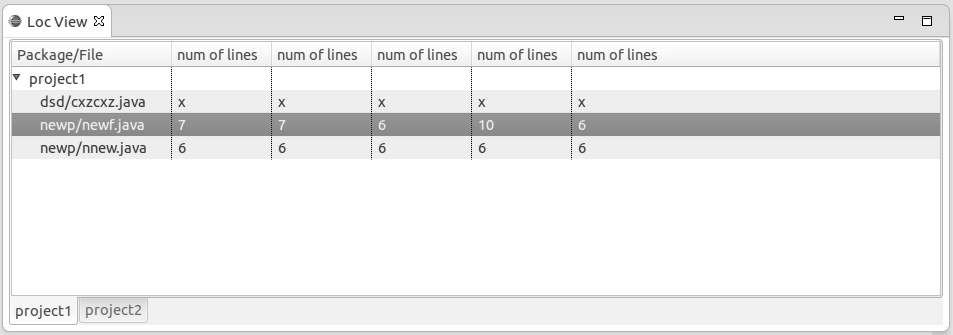
\includegraphics[width=\textwidth]{graphics/view.jpg}
	\caption{Widok na podstawowy wygl�d wtyczki.}
	\label{fig:view}
\end{figure}


\begin{figure}
	\centering
	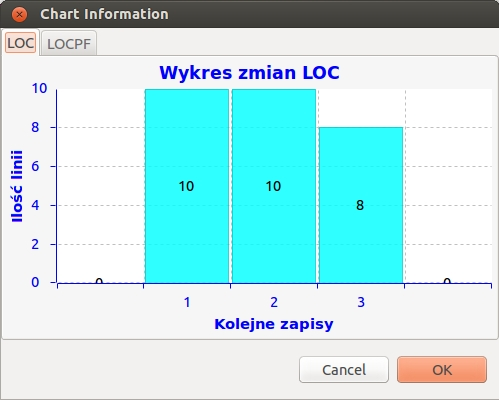
\includegraphics[width=\textwidth]{graphics/chartLOC.jpg}
	\caption{Widok na okno wykres�w LOC.}
	\label{fig:LOC}
\end{figure}


\begin{figure}
	\centering
	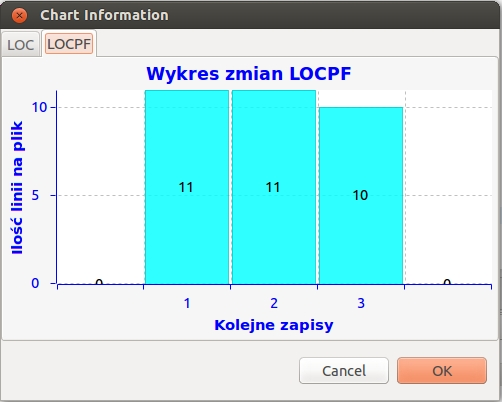
\includegraphics[width=\textwidth]{graphics/chartLOCPF.jpg}
	\caption{Widok na okno wykres�w LOCPF.}
	\label{fig:LOCPF}
\end{figure}





\bibliography{bibliografia01} 
\addcontentsline{toc}{section}{Bibliografia}

\end{document}
